% Formato de Informe para Sistemas de Información I
% Universidad Católica del Norte - Coquimbo
% Primer Semestre 2025

\documentclass[12pt,letterpaper]{report}

% Paquetes necesarios
\usepackage[spanish]{babel}
\usepackage[utf8]{inputenc}
\usepackage{graphicx}
\usepackage{fancyhdr}
\usepackage{hyperref}
\usepackage{booktabs}
\usepackage{tabularx}
\usepackage{xcolor}
\usepackage{enumitem}
\usepackage{titlesec}
\usepackage{float}

% Configuración de márgenes
\usepackage[top=2.5cm, bottom=2.5cm, left=3cm, right=3cm]{geometry}

% Configuración de títulos
\titleformat{\chapter}{\normalfont\LARGE\bfseries}{\thechapter.}{1em}{}
\titleformat{\section}{\normalfont\Large\bfseries}{\thesection}{1em}{}
\titleformat{\subsection}{\normalfont\large\bfseries}{\thesubsection}{1em}{}

% Configuración de encabezado y pie de página
\pagestyle{fancy}
\fancyhf{}
\fancyhead[L]{Sistemas de Información I}
\fancyhead[R]{Universidad Católica del Norte}
\fancyfoot[C]{\thepage}
\renewcommand{\headrulewidth}{0.4pt}
\renewcommand{\footrulewidth}{0.4pt}

% Configuración de hipervínculos
\hypersetup{
    colorlinks=true,
    linkcolor=blue,
    filecolor=magenta,      
    urlcolor=cyan,
    pdftitle={Proyecto de Sistemas de Información},
    pdfpagemode=FullScreen,
}

\begin{document}

%------------------------------------------------
% PORTADA
%------------------------------------------------
\begin{titlepage}
    \centering
    \vspace*{1cm}
    
\includegraphics[width=0.4\textwidth]{ucn-EIC.pdf}
    \vspace{1cm}
    
    {\LARGE \textbf{UNIVERSIDAD CATÓLICA DEL NORTE}}\\
    \vspace{0.5cm}
    {\large Escuela de Ingeniería}\\
    \vspace{0.3cm}
    {\large ICCI - ITI}\\
    \vspace{0.3cm}
    {\large Coquimbo}\\
    \vspace{1.5cm}
    
    {\Huge \textbf{Proyecto de Sistemas de Información}}\\
    \vspace{0.5cm}
    {\LARGE Sistemas de Información I}\\
    \vspace{1.5cm}
    
    {\large \textbf{Integrantes:}}\\
    \vspace{0.3cm}
    {\large Daniela Castro }
    {\large Vicente Espinoza }\\
    {\large Diego Martínez}\\
    {\large Sebastián Vega}\\
    {\large Gabriel Vergara}\\
    \vspace{1.5cm}
    
    {\large \textbf{Profesor:} Felipe Quiroz}\\
    \vspace{1.5cm}
    
    {\large Primer Semestre 2025}
    
\end{titlepage}

%------------------------------------------------
% ÍNDICE
%------------------------------------------------
\tableofcontents
\newpage

%------------------------------------------------
% INTRODUCCIÓN
%------------------------------------------------
\chapter*{Introducción}
\addcontentsline{toc}{chapter}{Introducción}

La formacion de profesionales es uno de los pilares principales para las universidades, para ello deben pasar un proceso riguroso de varios años para poder salir a un campo laboral a poder aplicar lo aprendido. Sin embargo, no todas las personas que entran a universiades y/o insitutos tienden a completar este proceso de educacion superior, donde el rendimiento de cada estudiante corresponde a una de las cuantas razones validas para que ocurra este suceso. Es por eso que la Universidad Catolica del Norte, comprometida con la excelencia educativa y academica, ha identificado la necesidad de analizar habitos y estilos de vida de los estudiantes de su institucion para determinar como estos impactan en su desempeño universitario.

Durante este proyecto, se busca abordar esta problematica mediante el análisis de un dataset simulado que contiene el registro de 1.000 estudiantes, con mas de 15 variables a analizar las cuales seran detalladas mas adelante. Para ello, se utilizaran tecnicas de analisis de datos, visualizacion en Power BI y KPIs relevantes. Esto permitira tomar decisiones informadas para impulsar y mejorar el desempeño estudiantil.

\newpage

%------------------------------------------------
% PASOS DEL PROYECTO
%------------------------------------------------
\chapter{Desarrollo del Proyecto}

%------------------------------------------------
% PASO 1: ANÁLISIS DE LA ORGANIZACIÓN
%------------------------------------------------
\section{Paso 1: Análisis de la Organización}

\subsection{Misión}
La Universidad Católica del Norte inspirada en los principios del Humanismo Cristiano y la misión de la Iglesia Católica, contribuye a la creación y transferencia del conocimiento, a la formación integral de la persona y el desarrollo tecnológico. Como institución con vocación de servicio y excelencia impulsa desde el Norte de Chile, con las comunidades y el territorio, la sostenibilidad a través de la docencia, investigación y vinculación con el medio.

\subsection{Visión}
Desde su identidad católica y vocación de excelencia, ser una universidad referente en su quehacer, que inspirada en el bien común integre disciplinas, tradiciones, culturas y comunidades para transformar vidas y ampliar oportunidades. 

\subsection{Descripción Detallada}
La Universidad Católica del Norte (UCN) fundada en el año 1956, es una institución privada de educación superior que reside en Chile, específicamente en las ciudades de Coquimbo y Antofagasta, siendo esta última ciudad donde se encuentra la sede principal. Esta universidad forma parte del Consejo de Rectores de las Universidades Chilenas (CRUCH) y de la Red G9, que agrupa a las principales universidades tradicionales no estatales del país. Cuenta actualmente con más de 50 carreras de pregrado, las cuales en su mayoría se encuentran en su sede principal, pero también ofrece programas de postgrado, magisteres, doctorados y diplomados

%------------------------------------------------
% PASO 2: INTRODUCCIÓN A LA PROBLEMÁTICA
%------------------------------------------------
\section{Paso 2: Introducción a la Problemática}

\subsection{Descripción del Problema}
Se identificó en la Universidad Católica del Norte que estudiantes de distintas facultades tenían bajo rendimiento académico lo que provocó que muchos abandonaran sus respectivas carreras o que se atrasaran varios años. Por lo cual se decidió investigar cuáles podrían ser las razones por las que esto ocurre con tanta frecuencia, para poder ponerle un freno a esta situación y ayudar a los estudiantes con herramientas para mejorar su desempeño. Por ello se contempló la posibilidad de trabajar con un dataset sintético para evaluar posibles causas de este problema y así poder presentar soluciones que resuelvan o mitiguen los efectos provocados por el bajo rendimiento de los estudiantes.
\subsection{Justificación}
Es relevante poner un énfasis en la resolución de la problemática mencionada, para lograr disminuir el porcentaje de reprobación en los estudiantes, para que así puedan culminar sus estudios en la duración establecida de su carrera. En promedio en Chile, los estudiantes se gradúan en 1,25 años más de la extensión real del pregrado. Además, se estimó que en la Universidad Católica del Norte los estudiantes se tardan entre 2 y 2,5 años en concluir sus estudios, al estar sobre el promedio del país, supone un problema real que afecta a los estudiantes de esta casa de estudios.
Gracias a la investigación, se espera poder identificar correctamente las causas fundamentales que generan esta problemática, para poder disminuir significativamente los años adicionales que requieren los alumnos para finalizar sus estudios, analizando estrategias de apoyo para eliminar o mitigar el efecto que producen las razones por las cuales su rendimiento se ve afectado, logrando así herramientas beneficiosas para fomentar el aprendizaje.

\subsection{Identificación de Stakeholders}
Los stakeholders del proyecto representan los grupos de interés clave que se verán impactados por el sistema de información a desarrollar. En el contexto de la Universidad Católica del Norte, se han identificado cuatro grupos principales que tienen diferentes roles y expectativas respecto al proyecto de análisis de hábitos y rendimiento estudiantil.

\begin{table}[H]
    \centering
    \begin{tabularx}{\textwidth}{|X|X|X|}
        \hline
        \textbf{Stakeholder} & \textbf{Rol/Relación} & \textbf{Intereses/Expectativas} \\
        \hline
        Estudiantes & Usuarios principales del sistema educativo y sujetos de análisis & Mejorar su rendimiento académico, recibir retroalimentación sobre sus hábitos de estudio, obtener recomendaciones para optimizar su desempeño académico \\
        \hline
        Egresados & Ex-estudiantes que formaron parte de la universidad & Contribuir con su experiencia para mejorar la formación de las futuras generaciones \\
        \hline
        Personal Administrativo & Responsables de la gestión académica y servicios estudiantiles & Contar con herramientas para el seguimiento estudiantil y tomar decisiones basadas en datos para mejorar servicios \\
        \hline
        Académicos & Docentes que forman parte del proceso educativo & Mejorar metodologías de enseñanza basado en resultados obtenidos \\
        \hline
    \end{tabularx}
    \caption{Identificación de Stakeholders}
\end{table}

\begin{figure}[!ht]
    \centering
    \includegraphics[width=1.2\textwidth]{stakeholders.png}
    \caption{Stakeholders}
    \label{fig:grafico1}
\end{figure}

%------------------------------------------------
% PASO 3: IDENTIFICACIÓN Y DETALLE DEL PROCESO
%------------------------------------------------
\section{Paso 3: Identificación y Detalle del Proceso}

\subsection{Descripción General del Proceso}
El proceso a trabajar consiste en el diseño, desarrollo y aplicación de un sistema de análisis de información basado en datos estudiantiles, que permita identificar patrones y factores que influyen en el bajo rendimiento académico de los estudiantes. El sistema utilizará un dataset sintético que representa los hábitos de estudio, salud mental, actividades extracurriculares y otros factores, para luego correlacionarlos con el rendimiento académico.

Este proceso se enmarca dentro de un proyecto de inteligencia de negocios académica, en el que se busca transformar datos en conocimiento útil para la toma de decisiones en contextos educativos.

\subsection{Diagrama del Proceso}

\begin{figure}
    \centering
    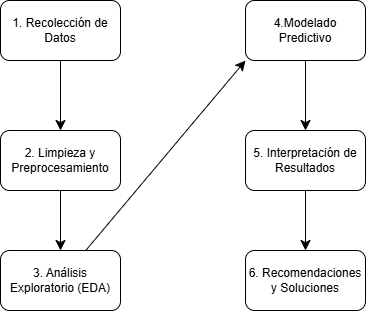
\includegraphics[width=0.5\linewidth]{diagrama de flujo.drawio.png}
    \caption{Diagrama de flujo del proceso}
    \label{fig:enter-label}
\end{figure}

\subsection{Detalle de Cada Paso del Proceso}

\begin{table}[H]
    \centering
    \renewcommand{\arraystretch}{1.3}
    \begin{tabular}{|p{3cm}|p{5cm}|p{3cm}|p{5cm}|}
        \hline
        \textbf{Paso} & \textbf{Descripción} & \textbf{Responsable} & \textbf{Recursos necesarios} \\
        \hline
        Recolección de Datos &
        Obtención y comprensión del dataset sintético con variables relacionadas a hábitos estudiantiles y rendimiento. &
        Vicente Espinoza &
        Acceso a Kaggle, herramientas para visualizar CSV . \\
        \hline
        Limpieza y Preprocesamiento &
        Depuración de datos, tratamiento de valores faltantes y codificación de variables. &
        Daniela Castro &
        Python , Google Colab o Jupyter Notebook, documentación del dataset. \\
        \hline
        Análisis Exploratorio de Datos (EDA) &
        Identificación de patrones, correlaciones y visualización de relaciones entre variables. &
        Gabriel Vergara &
        Python , entorno de desarrollo , herramientas estadísticas básicas. \\
        \hline
        Modelado Predictivo &
        Aplicación de algoritmos de Machine Learning para predecir rendimiento académico. &
        Diego Martínez &
        Scikit-learn, XGBoost u otros modelos de ML, recursos computacionales , librerías de evaluación . \\
        \hline
        Interpretación de Resultados &
        Evaluación del modelo, análisis de métricas y extracción de insights clave. &
        Sebastián Vega &
        Documentación de métricas , visualizaciones de importancia de variables, herramientas de reporte . \\
        \hline
        Recomendaciones y Desarrollo de Soluciones &
        Elaboración de propuestas prácticas basadas en los resultados obtenidos para apoyar a estudiantes. &
        Daniela Castro &
        Resultados del análisis, documento de propuestas. \\
        \hline
    \end{tabular}
    \caption{Detalle de los Pasos del Proceso}
\end{table}


%------------------------------------------------
% PASO 4: IDENTIFICACIÓN DE PROBLEMA O MEJORA
%------------------------------------------------
\section{Paso 4: Identificación de Problema o Mejora}

\subsection{Árbol de Problemas}

El árbol de problemas es una herramienta de análisis que permite identificar y visualizar de manera estructurada un problema central, sus causas y sus efectos. Esta metodología facilita la comprensión integral de la problemática al establecer relaciones causales entre diferentes factores, permitiendo así un enfoque más efectivo para el diseño de soluciones.

En el contexto del rendimiento académico estudiantil de la Universidad Católica del Norte, se ha identificado como problema central: \textbf{"Rendimiento académico insuficiente en estudiantes de la Universidad Católica del Norte"}.

\subsubsection{Causas del Problema}

\textbf{Causas Directas:}
\begin{itemize}
    \item Hábitos de estudio inadecuados.
    \item Baja asistencia a clases.
    \item Deficiente gestión del tiempo.
    \item Falta de apoyo académico personalizado.
\end{itemize}

\textbf{Causas Indirectas:}

\textbf{\textit{Factores de Estilo de Vida:}}
\vspace{0.1cm}
\begin{itemize}
    \item Excesivo tiempo en redes sociales y entretenimiento digital.
    \item Horarios de sueño irregulares o insuficientes.
    \item Mala calidad de alimentación.
    \item Sedentarismo y falta de ejercicio.
\end{itemize}

\textbf{\textit{Factores Socioeconómicos:}}
\vspace{0.1cm}
\begin{itemize}
    \item Necesidad de trabajar medio tiempo.
    \item Limitado acceso a tecnología de calidad.
    \item Bajo nivel educativo de los padres.
    \item Estrés financiero familiar.
\end{itemize}

\textbf{\textit{Factores Institucionales:}}
\vspace{0.1cm}
\begin{itemize}
    \item Sistemas de seguimiento académico limitados.
    \item Falta de identificación temprana de estudiantes en riesgo.
    \item Insuficiente orientación en técnicas de estudio.
\end{itemize}

\subsubsection{Efectos del Problema}

\textbf{Efectos Directos:}
\vspace{0.1cm}
\begin{itemize}
    \item Bajas calificaciones en exámenes.
    \item Alto índice de reprobación de asignaturas.
    \item Deterioro de la salud mental estudiantil.
    \item Desmotivación académica.
\end{itemize}

\textbf{Efectos Indirectos:}
\vspace{0.1cm}
\begin{itemize}
    \item Aumento de la deserción universitaria.
    \item Reducción de la empleabilidad de egresados.
    \item Deterioro del prestigio institucional.
    \item Pérdida de recursos económicos.
\end{itemize}

\subsection{Matriz de Vester}

La Matriz de Vester es una herramienta de análisis que permite evaluar la influencia que ejercen los diferentes problemas identificados entre sí, facilitando su priorización según su grado de motricidad y dependencia. Esta metodología clasifica los problemas en cuatro categorías: críticos, activos, pasivos e indiferentes, permitiendo enfocar los esfuerzos en aquellos que generarán mayor impacto.

Para el análisis del rendimiento académico estudiantil, se han identificado los siguientes problemas:

\begin{itemize}
    \item \textbf{P1}: Hábitos de estudio inadecuados.
    \item \textbf{P2}: Excesivo uso de redes sociales y entretenimiento.
    \item \textbf{P3}: Horarios de sueño irregulares.
    \item \textbf{P4}: Falta de ejercicio físico.
    \item \textbf{P5}: Necesidad de trabajar medio tiempo.
    \item \textbf{P6}: Limitado acceso a tecnología.
    \item \textbf{P7}: Bajo apoyo familiar en educación.
    \item \textbf{P8}: Sistema de seguimiento académico limitado.
\end{itemize}

\begin{table}[H]
    \centering
    \begin{tabular}{|c|c|c|c|c|c|c|c|c|c|}
        \hline
        \textbf{Problemas} & \textbf{P1} & \textbf{P2} & \textbf{P3} & \textbf{P4} & \textbf{P5} & \textbf{P6} & \textbf{P7} & \textbf{P8} & \textbf{Total Activos} \\
        \hline
        \textbf{P1} & 0 & 2 & 3 & 1 & 1 & 1 & 0 & 0 & \textbf{8} \\
        \hline
        \textbf{P2} & 3 & 0 & 3 & 2 & 0 & 0 & 0 & 0 & \textbf{8} \\
        \hline
        \textbf{P3} & 3 & 1 & 0 & 2 & 1 & 0 & 0 & 0 & \textbf{7} \\
        \hline
        \textbf{P4} & 2 & 0 & 1 & 0 & 0 & 0 & 0 & 0 & \textbf{3} \\
        \hline
        \textbf{P5} & 2 & 1 & 2 & 3 & 0 & 0 & 1 & 0 & \textbf{9} \\
        \hline
        \textbf{P6} & 1 & 0 & 0 & 0 & 0 & 0 & 0 & 1 & \textbf{2} \\
        \hline
        \textbf{P7} & 2 & 0 & 1 & 1 & 2 & 3 & 0 & 0 & \textbf{9} \\
        \hline
        \textbf{P8} & 1 & 0 & 0 & 0 & 0 & 0 & 0 & 0 & \textbf{1} \\
        \hline
        \textbf{Total Pasivos} & \textbf{14} & \textbf{4} & \textbf{10} & \textbf{9} & \textbf{4} & \textbf{4} & \textbf{1} & \textbf{1} & \\
        \hline
    \end{tabular}
    \caption{Matriz de Vester - Influencia entre Problemas del Rendimiento Académico}
\end{table}

\subsubsection{Clasificación de Problemas según Matriz de Vester}

\textbf{Problemas Críticos (Alto Activo, Alto Pasivo):}
\begin{itemize}
    \item P1: Hábitos de estudio inadecuados (8,14).
    \item P3: Horarios de sueño irregulares (7,10).
\end{itemize}

\textbf{Problemas Activos (Alto Activo, Bajo Pasivo):}
\begin{itemize}
    \item P5: Necesidad de trabajar medio tiempo (9,4).
    \item P7: Bajo apoyo familiar en educación (9,1).
\end{itemize}

\textbf{Problemas Pasivos (Bajo Activo, Alto Pasivo):}
\begin{itemize}
    \item P4: Falta de ejercicio físico (3,9).
\end{itemize}

\textbf{Problemas Indiferentes (Bajo Activo, Bajo Pasivo):}
\begin{itemize}
    \item P2: Excesivo uso de redes sociales (8,4).
    \item P6: Limitado acceso a tecnología (2,4).
    \item P8: Sistema de seguimiento limitado (1,1).
\end{itemize}

\subsection{Cadena de Valor}

La cadena de valor es un modelo que describe las actividades de una organización para generar valor al cliente final. Desarrollada por Michael Porter, esta herramienta permite identificar las actividades primarias y de apoyo que contribuyen a la ventaja competitiva. En el contexto universitario, la cadena de valor nos ayuda a entender cómo el proceso de rendimiento académico estudiantil se integra con las diferentes actividades institucionales y dónde se pueden implementar mejoras.

\subsubsection{Actividades Primarias de la UCN}

\textbf{Docencia (Enseñanza-Aprendizaje):}
\begin{itemize}
    \item \textbf{\textit{Ubicación del proceso}:} El rendimiento académico es el resultado directo de esta actividad.
    \item \textbf{\textit{Impacto}:} Directamente afectado por la calidad de los procesos de seguimiento y apoyo estudiantil.
    \item \textbf{\textit{Oportunidad de mejora}:} Implementación de sistemas de monitoreo continuo del progreso académico.
\end{itemize}

\textbf{Investigación:}
\begin{itemize}
    \item \textbf{\textit{Relación}:} Los estudiantes con mejor rendimiento pueden participar más activamente en proyectos de investigación.
    \item \textbf{\textit{Impacto}:} El bajo rendimiento limita la participación estudiantil en actividades de investigación.
    \item \textbf{\textit{Oportunidad}:} Usar la investigación como herramienta motivacional para mejorar el rendimiento.
\end{itemize}

\textbf{Vinculación con el Medio:}
\begin{itemize}
    \item \textbf{\textit{Relación}:} El rendimiento académico afecta la calidad de los profesionales que se vinculan con el entorno.
    \item \textbf{\textit{Impacto}:} Estudiantes con mejor rendimiento representan mejor a la universidad en actividades externas.
    \item \textbf{\textit{Oportunidad}:} Establecer programas de vinculación que motiven el mejor rendimiento académico.
\end{itemize}

\subsubsection{Actividades de Apoyo de la UCN}

\textbf{Gestión de Recursos Humanos:}
\begin{itemize}
    \item \textbf{\textit{Relación}:} Formación docente en técnicas de seguimiento académico y detección temprana de problemas.
    \item \textbf{\textit{Oportunidad}:} Capacitación especializada en metodologías de apoyo estudiantil personalizado.
\end{itemize}

\textbf{Desarrollo Tecnológico:}
\begin{itemize}
    \item \textbf{\textit{Relación}:} Sistemas de información para seguimiento académico y análisis predictivo.
    \item \textbf{\textit{Oportunidad}:} Implementación de analytics educativo para predecir y prevenir bajo rendimiento.
\end{itemize}

\textbf{Infraestructura:}
\begin{itemize}
    \item \textbf{\textit{Relación}:} Espacios de estudio, bibliotecas, laboratorios y tecnología disponible.
    \item \textbf{\textit{Impacto}:} La calidad de infraestructura afecta directamente las condiciones de estudio.
\end{itemize}

\textbf{Adquisiciones:}
\begin{itemize}
    \item \textbf{\textit{Relación}:} Recursos tecnológicos, bibliográficos y herramientas de apoyo académico.
    \item \textbf{\textit{Oportunidad}:} Inversión estratégica en herramientas de seguimiento y apoyo estudiantil.
\end{itemize}

\subsection{Análisis FODA}

El análisis FODA es una herramienta de diagnóstico estratégico que permite evaluar la situación interna y externa de una organización. En el contexto del rendimiento académico estudiantil, el FODA nos ayuda a identificar los elementos internos y externos que influyen en esta problemática y a desarrollar estrategias específicas para su mejora.

\begin{table}[H]
    \centering
    \begin{tabular}{|p{0.45\textwidth}|p{0.45\textwidth}|}
        \hline
        \textbf{Fortalezas} & \textbf{Oportunidades} \\
        \hline
        \begin{itemize}
            \item Prestigio y trayectoria de 60+ años en educación superior.
            \item Enfoque humanista cristiano que promueve formación integral.
            \item Ubicación estratégica en el norte de Chile.
            \item Cuerpo académico calificado con experiencia.
            \item Infraestructura tecnológica en desarrollo.
            \item Programas acreditados y reconocidos.
            \item Cultura organizacional orientada a las personas.
        \end{itemize} & 
        \begin{itemize}
            \item Creciente demanda de educación superior en la región.
            \item Avances tecnológicos en analytics educativo y big data.
            \item Políticas gubernamentales de apoyo a la educación superior.
            \item Alianzas estratégicas con organizaciones públicas y privadas.
            \item Desarrollo de metodologías de enseñanza innovadoras.
            \item Programas de bienestar estudiantil en expansión.
            \item Tendencia hacia la personalización educativa.
        \end{itemize} \\
        \hline
        \textbf{Debilidades} & \textbf{Amenazas} \\
        \hline
        \begin{itemize}
            \item Limitado sistema de seguimiento individual del rendimiento académico.
            \item Falta de identificación temprana de estudiantes en riesgo.
            \item Limitada integración de datos estudiantiles para análisis predictivo.
            \item Recursos limitados para programas de bienestar estudiantil.
            \item Falta de capacitación docente en seguimiento académico.
            \item Sistemas de información académica no integrados.
        \end{itemize} & 
        \begin{itemize}
            \item Competencia creciente de otras universidades en la región.
            \item Cambios socioeconómicos que afectan el acceso a educación superior.
            \item Impacto de factores externos en el bienestar estudiantil.
            \item Limitaciones presupuestarias del sector educativo.
            \item Rápidos cambios tecnológicos que requieren constante actualización.
            \item Expectativas crecientes de estudiantes y empleadores.
            \item Factores socioeconómicos familiares que afectan el rendimiento.
        \end{itemize} \\
        \hline
    \end{tabular}
    \caption{Análisis FODA - Rendimiento Académico Estudiantil UCN}
\end{table}

\subsubsection{Estrategias Derivadas del Análisis FODA}

\textbf{Estrategias FO (Fortalezas + Oportunidades):}
\begin{itemize}
    \item Aprovechar el prestigio institucional y los avances tecnológicos para desarrollar un sistema líder en seguimiento académico en la región.
    \item Utilizar la cultura orientada a personas y las metodologías innovadoras para personalizar el apoyo estudiantil.
    \item Capitalizar la ubicación estratégica y las alianzas para crear programas de apoyo integral únicos en el norte de Chile.
\end{itemize}

\textbf{Estrategias FA (Fortalezas + Amenazas):}
\begin{itemize}
    \item Usar la trayectoria institucional y programas acreditados para diferenciarse de la competencia creciente.
    \item Aprovechar el enfoque humanista para contrarrestar factores socioeconómicos adversos que afectan a los estudiantes.
    \item Utilizar el cuerpo académico calificado para adaptarse rápidamente a los cambios tecnológicos.
\end{itemize}

\textbf{Estrategias DO (Debilidades + Oportunidades):}
\begin{itemize}
    \item Desarrollar sistemas integrados de seguimiento académico aprovechando los avances en analytics educativo.
    \item Implementar programas de apoyo personalizado usando las políticas gubernamentales de apoyo disponibles.
    \item Capacitar al personal docente en metodologías innovadoras para la identificación temprana de problemas académicos.
\end{itemize}

\textbf{Estrategias DA (Debilidades + Amenazas):}
\begin{itemize}
    \item Fortalecer los sistemas de información académica para responder mejor a las expectativas crecientes de estudiantes y empleadores.
    \item Mejorar la capacitación docente y los programas de bienestar para enfrentar los cambios tecnológicos y socioeconómicos.
    \item Desarrollar alianzas estratégicas para compensar las limitaciones presupuestarias y de recursos.
\end{itemize}

%------------------------------------------------
% PASO 5: DEFINICIÓN DE OBJETIVOS, ALCANCE Y SOLUCIÓN
%------------------------------------------------
\section{Paso 5: Definición de Objetivos, Alcance y Solución}

\subsection{Objetivos}

\subsubsection{Objetivo General}
Desarrollar un sistema predictivo para evaluar cómo los hábitos de vida estudiantil influyen en el 
rendimiento académico, permitiendo la identificación temprana de estudiantes en riesgo y la 
implementación de estrategias de intervención en la Universidad Católica del Norte.

\subsubsection{Objetivos Específicos}
\begin{itemize}
\item Establecer correlaciones estadísticas entre variables de estilo de vida (patrones de sueño, uso de redes sociales, hábitos alimenticios, actividad física) y el desempeño en exámenes finales
\item Construir modelos predictivos que permitan anticipar el rendimiento académico individual basándose en indicadores comportamentales
\item Identificar perfiles de riesgo académico mediante técnicas de clustering para segmentar estudiantes según sus patrones de comportamiento
\item Cuantificar el impacto relativo de cada factor de estilo de vida en el éxito académico estudiantil
\item Generar recomendaciones basadas en datos para optimizar los hábitos que más contribuyen al rendimiento académico
\item Desarrollar un dashboard interactivo para el seguimiento continuo y la toma de decisiones académicas
\end{itemize}

\subsection{Alcance}
\textbf{Dentro del alcance:}
\begin{itemize}
\item Análisis del dataset simulado con 1,000 registros estudiantiles y 15+ variables comportamentales
\item Implementación de algoritmos de machine learning supervisado para predicción de calificaciones
\item Aplicación de técnicas de clustering no supervisado para identificación de patrones estudiantiles
\item Evaluación comparativa de múltiples modelos predictivos (regresión, árboles de decisión, ensemble methods)
\item Análisis de importancia de características para identificar factores críticos
\end{itemize}
\textbf{Fuera del alcance:}
\begin{itemize}
\item Recopilación de información primaria de estudiantes reales de la UCN
\item Implementación de sistemas de monitoreo en tiempo real en la infraestructura universitaria
\item Desarrollo de aplicaciones móviles o plataformas de producción
\item Análisis de variables externas como condiciones familiares
\end{itemize}

\subsection{Descripción de la Solución Propuesta}
La propuesta consiste en el desarrollo de un sistema analítico que utiliza técnicas de ciencia de datos para transformar 
información sobre hábitos estudiantiles en insights accionables para mejorar el rendimiento académico institucional.
\vspace{0.3cm}

\textbf{Arquitectura de la solución:}

\vspace{0.3cm}
\textbf{1. Módulo de Preprocesamiento de Datos:} Limpieza, normalización y preparación del dataset, incluyendo tratamiento de valores atípicos y transformación de variables categóricas para optimizar el análisis.
\vspace{0.3cm}

\textbf{2. Motor de Análisis Exploratorio:} Implementación de técnicas estadísticas descriptivas e inferenciales para descubrir patrones ocultos, correlaciones significativas y distribuciones relevantes en los datos comportamentales.
\vspace{0.3cm}

\textbf{3. Interface de Visualización y Reporting:} Creación de un dashboard interactivo que permita explorar resultados, generar predicciones individuales y visualizar tendencias mediante gráficos dinámicos y reportes personalizables.
\vspace{0.3cm}

\textbf{Valor agregado de la solución:} La implementación proporcionará a la Universidad herramientas de análisis que faciliten decisiones fundamentadas en datos reales. 
La solución permitirá detectar oportunamente a estudiantes que puedan presentar dificultades académicas, optimizar el uso de recursos destinados al apoyo estudiantil y 
ofrecer sugerencias basadas en comportamientos que han demostrado generar buenos resultados.


%------------------------------------------------
% PASO 6: PLANIFICACIÓN
%------------------------------------------------
\section{Paso 6: Planificación}

\subsection{Ciclo de Desarrollo}
Se empleará el ciclo de desarrollo incremental, ideal para proyectos de análisis de datos donde se puede trabajar en etapas parciales que se mejoran progresivamente. Este ciclo permite entregar avances funcionales desde etapas tempranas, realizar retroalimentación continua y ajustar soluciones conforme se avanza en el análisis.
\begin{enumerate}
    \item Recolección y comprensión inicial de datos
    \item Primer análisis y visualización
    \item Construcción de modelos iniciales
    \item Validación y ajuste de modelos
    \item Extracción de resultados y generación de propuestas
    \item Documentación y presentación
\end{enumerate}

\subsection{División del Trabajo y Roles del Equipo}

\begin{table}[H]
    \centering
    \begin{tabularx}{\textwidth}{|X|X|X|}
        \hline
        \textbf{Miembro del Equipo} & \textbf{Rol} & \textbf{Responsabilidades} \\
        \hline Daniela Castro
        & Coordinadora del Proyecto & Coordina reuniones, lidera la integración de entregables y revisa avances finales. \\
        \hline Vicente Espinoza
        & Encargado de Datos & Descarga, organiza y documenta el dataset. Prepara los datos para su análisis.\\
        \hline Gabriel Vergara
        & Analista Exploratorio & Realiza el análisis exploratorio y genera visualizaciones para detectar patrones.\\
        \hline Diego Martínez
        & Modelador de Datos & Desarrolla modelos predictivos y evalúa su rendimiento con métricas adecuadas.\\
        \hline Sebastián Vega
        & Evaluador y Documentador & Interpreta resultados del modelo, redacta conclusiones y elabora las recomendaciones.\\
        \hline
    \end{tabularx}
    \caption{Roles y Responsabilidades del Equipo}
\end{table}

\subsection{Tareas y Plazos}
[Definir las tareas específicas del proyecto y establecer plazos para su realización]

\begin{table}[H]
    \centering
    \begin{tabularx}{\textwidth}{|X|X|X|X|X|}
        \hline
        \textbf{Tarea} & \textbf{Responsable} & \textbf{Fecha Inicio} & \textbf{Fecha Fin} & \textbf{Dependencias} \\
        \hline  Primer informe y presentación de avance
        & Todo el equipo & 18 Mayo & 23 Mayo& \\
        \hline Recolección y organización de datos 
        & Vicente Espinoza & 23 Mayo & 27 Mayo& Dataset\\
        \hline Limpieza y preprocesamiento de datos
        & Daniela Castro & 	27 Mayo & 31 Mayo & Recolección de datos \\
        \hline Análisis exploratorio y visualizaciones
        & Gabriel Vergara & 1 Junio & 7 Junio & Preprocesamiento de datos \\
        \hline Desarrollo de modelo predictivo inicial
        & Diego Martínez & 8 Junio & 12 Junio&Análisis exploratorio\\
        \hline Evaluación del modelo y ajuste
        & Diego Martínez & 10 Junio & 14 Junio &  Modelo inicial\\
        \hline Interpretación y generación de propuestas
        & Sebastián Vega & 14 Junio & 20 Junio & Modelo validado\\
        \hline Redacción de informe final
        & Todo el equipo & 20 Junio & 28 Junio& Todos los pasos anteriores\\
        \hline Preparación presentación final
        & Todo el equipo & 28 Junio & 30 Junio& Informe y resultados finales \\
        \hline
    \end{tabularx}
    \caption{Cronograma de Tareas}
\end{table}

%------------------------------------------------
% PASO 7: IDENTIFICACIÓN DE KPI
%------------------------------------------------
\section{Paso 7: Identificación de KPI}

\subsection{Definición de KPI}
Los siguientes KPIs fueron seleccionados para evaluar el rendimiento académico de los estudiantes y su relación con sus hábitos diarios.

\begin{table}[H]
    \centering
    \begin{tabularx}{\textwidth}{|X|X|X|X|X|}
        \hline
        \textbf{KPI} & \textbf{Descripción} & \textbf{Fórmula de Cálculo} & \textbf{Meta} & \textbf{Impacto en el Proceso} \\
        \hline
        Puntaje promedio (AvgScore) & Mide el rendimiento académico promedio de todos los estudiantes en el examen. & Promedio de \texttt{exam\_score} & \textgreater 60 puntos & Permite evaluar si el rendimiento general es adecuado o si se requiere reforzar contenidos. \\
        \hline
        Porcentaje de alumnos aprobados & Indica el porcentaje de estudiantes que superan el 60\% de exigencia impartido por la Universidad Católica del Norte & Se calcula el porcentaje de estudiantes que tienen un \texttt{exam\_score} mayor a 60\% & \textgreater 75\% & Identifica el grado de éxito académico y permite detectar necesidades de intervención educativa. \\
        \hline
        Promedio de horas de estudio por día & Refleja las horas promedio de estudio de los estudiantes & Promedio de \texttt{study\_hours\_per\_day} & 2 a 4 horas & Ayuda a correlacionar hábitos de estudio con el rendimiento, detectando si el tiempo invertido es eficiente. \\
        \hline
        Promedio de horas de sueño & Indica el promedio de descanso de los estudiantes. & Promedio de \texttt{sleep\_hours} & 7 a 9 horas & Permite evaluar el impacto del descanso en el rendimiento académico. \\
        \hline
    \end{tabularx}
    \caption{Indicadores Clave de Desempeño (KPI)}
\end{table}

\subsection{Justificación de los KPI Seleccionados}
Los KPI seleccionados permiten identificar de manera objetiva y cuantificable el nivel de rendimiento académico general de los estudiantes y su relación con factores clave como el tiempo de estudio y el descanso. La elección de estos indicadores está alineada con los objetivos del proyecto, ya que permite detectar patrones que afectan el desempeño y, con ello, generar recomendaciones prácticas para mejorar el aprendizaje.

%------------------------------------------------
% PASO 8: DEFINICIÓN Y DESCRIPCIÓN DE LOS DATOS
%------------------------------------------------
\section{Paso 8: Definición y Descripción de los Datos}

\section{Descripción del Data Set}
El dataset seleccionado revela con datos sintéticos los hábitos de 1.000 estudiantes, considerando 14 variables entre las cuales se encuentra; edad, género, horas de estudio por día, horas dedicadas a redes sociales, horas de netflix, porcentaje de asistencia, horas de sueño, calidad de alimentación, frecuencia de ejercicio, nivel de educación de los padres, calidad de internet, evaluación de salud mental (escala del 1 al 10), participación en actividades extracurriculares, trabajo tiempo parcial (si o no), para evaluar la influencia de dichos indicadores en el puntaje de sus exámenes
Se encuentra en formato .csv, donde las columnas corresponden a las variables, siendo la última de éstas, las calificaciones y las filas las respuestas de los estudiantes. De las categorías mencionadas anteriormente se tienen 9 variables cuantitativas (de las cuales 3 son discretas y 6 son continuas) y 5 variable cualitativas (3 nominales y 2 ordinales)

\section{Justificación del Data Set}
La elección del análisis del actual dataset representa una herramienta para analizar cómo los hábitos de los estudiantes pueden afectar el rendimiento académico, sirviendo para comparar cuáles variables podrían incidir en los resultados de los exámenes finales de los estudiantes. Es de suma importancia hacer un énfasis en esta investigación para determinar como aumentar el rendimiento de los estudiantes y posteriormente aplicar las herramientas encontradas para aplicarlas a un grupo de personas real, contribuyendo así a una mejora de los hábitos de ellos.

\section{Calidad y Limitaciones de los Datos}
En el dataset no se presentan datos faltantes. En cuanto a inconsistencias, aparentemente no se encontró ninguna, pero si podría generar dudas para el análisis, el hecho de que existan al menos 12 estudiantes que estudian 0 horas diarias, y un estudiante que trabaja part time, que estudia 8.3 horas, duerme 6.5, obtiene 100 de puntaje en el examen y posee tiempo para redes sociales y netflix, ya que los tiempos no coinciden por completo, lo cual podría indicar falsedad en la respuesta del estudiante.
Una limitación que podría presentar el set de datos corresponde a la cantidad de información presentada, debido a que sólo se tienen 1.000 estudiantes, se podría haber tomado un valor mayor o haber indicado que los estudiantes corresponden a una facultad en específico, para así tener un mayor panorama de otras variables que podrían influenciar negativamente en la precisión del estudio. Otro aspecto a considerar sería el incluir las razones de las inasistencias, ya que se podría llegar a una conclusión errónea, como por ejemplo decir que los estudiantes por irresponsabilidad (por el hecho de no asistir a clases) no obtuvieron un buen rendimiento en el examen, cuando pueden haberse ausentado por enfermedad. Y,
finalmente agregar el tipo de actividad extracurricular que realizan los estudiantes, ya que esto facilitaría establecer una conexión de actividades extracurriculares que ayudan a los estudiantes a mejorar su rendimiento.

%------------------------------------------------
% PASO 9: PREPARACIÓN DE LOS DATOS
%------------------------------------------------
\section{Paso 9: Preparación de los Datos}

\subsection{Carga de Datos}
Los datos fueron cargados a Power BI desde un archivo en formato \texttt{.csv}, el cual tenía información estructurada tal como se detalló en la sección \textbf{Definición Data Set} La importación se realizó mediante la funcionalidad de "Obtener datos", seleccionando el tipo "Archivo CSV", y posteriormente se inspeccionaron los encabezados y tipos de datos detectados por Power BI. Durante esta etapa se verificó la correcta codificación del archivo (UTF-8) y se ajustaron los delimitadores en caso de ser necesario.

\subsection{Transformación de Datos}
Se realizaron validaciones sobre cada variable, para asegurar que sus valores estuvieran dentro de los rangos establecidos. 
Se agregó un campo calculado llamado \texttt{total\_daily\_hours}, el cual suma las horas indicadas de sueño, estudio, Netflix, redes sociales, 4 horas estimadas para los estudiantes que indicaron tener un trabajo part time, y una estimación adicional de las horas de clases basada en el porcentaje de asistencia. En concreto, se estableció que el 80\%, 50\% y 20\% corresponden a 6, 3 y 1 horas de clase respectivamente.  
A continuación, se muestra el desglose de las variables originales transformadas, junto con las variables resultantes.

\begin{table}[H]
    \centering
    \begin{tabularx}{\textwidth}{|l|X|l|}
        \hline
        \textbf{Variable Original} & \textbf{Transformación Aplicada} & \textbf{Variable Resultante} \\
        \hline
        \texttt{study\_hours\_per\_day}, \texttt{sleep\_hours}, \texttt{social\_media\_hours}, \texttt{netflix\_hours}, \texttt{part\_time\_job}, \texttt{attendance\_percentage} & Se creó una columna que suma horas de estudio, sueño, ocio, trabajo part-time (si aplica) y tiempo académico estimado en función de la asistencia. Esta transformación permitió detectar registros cuyo total diario excedía las 24 horas. & \texttt{total\_daily\_hours} \\
        \hline
        \texttt{total\_daily\_hours} & Se filtraron las filas donde el total de horas diarias superaba 24, eliminando registros con inconsistencias lógicas. & Filtrado (sin nueva variable) \\
        \hline
        \texttt{attendance\_percentage}, \texttt{sleep\_hours}, \texttt{study\_hours\_per\_day} & Se dividieron por 10 para normalizar los valores, ya que venían escalados incorrectamente. & Mismos nombres normalizados \\
        \hline
        \texttt{exam\_score} & Se dividió por 10 para ajustar la escala al rango correcto. & \texttt{exam\_score} (ajustado) \\
        \hline
    \end{tabularx}
    \caption{Transformaciones aplicadas durante la limpieza y validación de datos en Power BI}
\end{table}

Cabe destacar que la columna \texttt{total\_daily\_hours} fue generada únicamente con el fin de validar los datos y, por consiguiente, al finalizar el proceso de filtrado, fue eliminada para evitar redundancia en el modelo.

\begin{figure}[H]
    \centering
    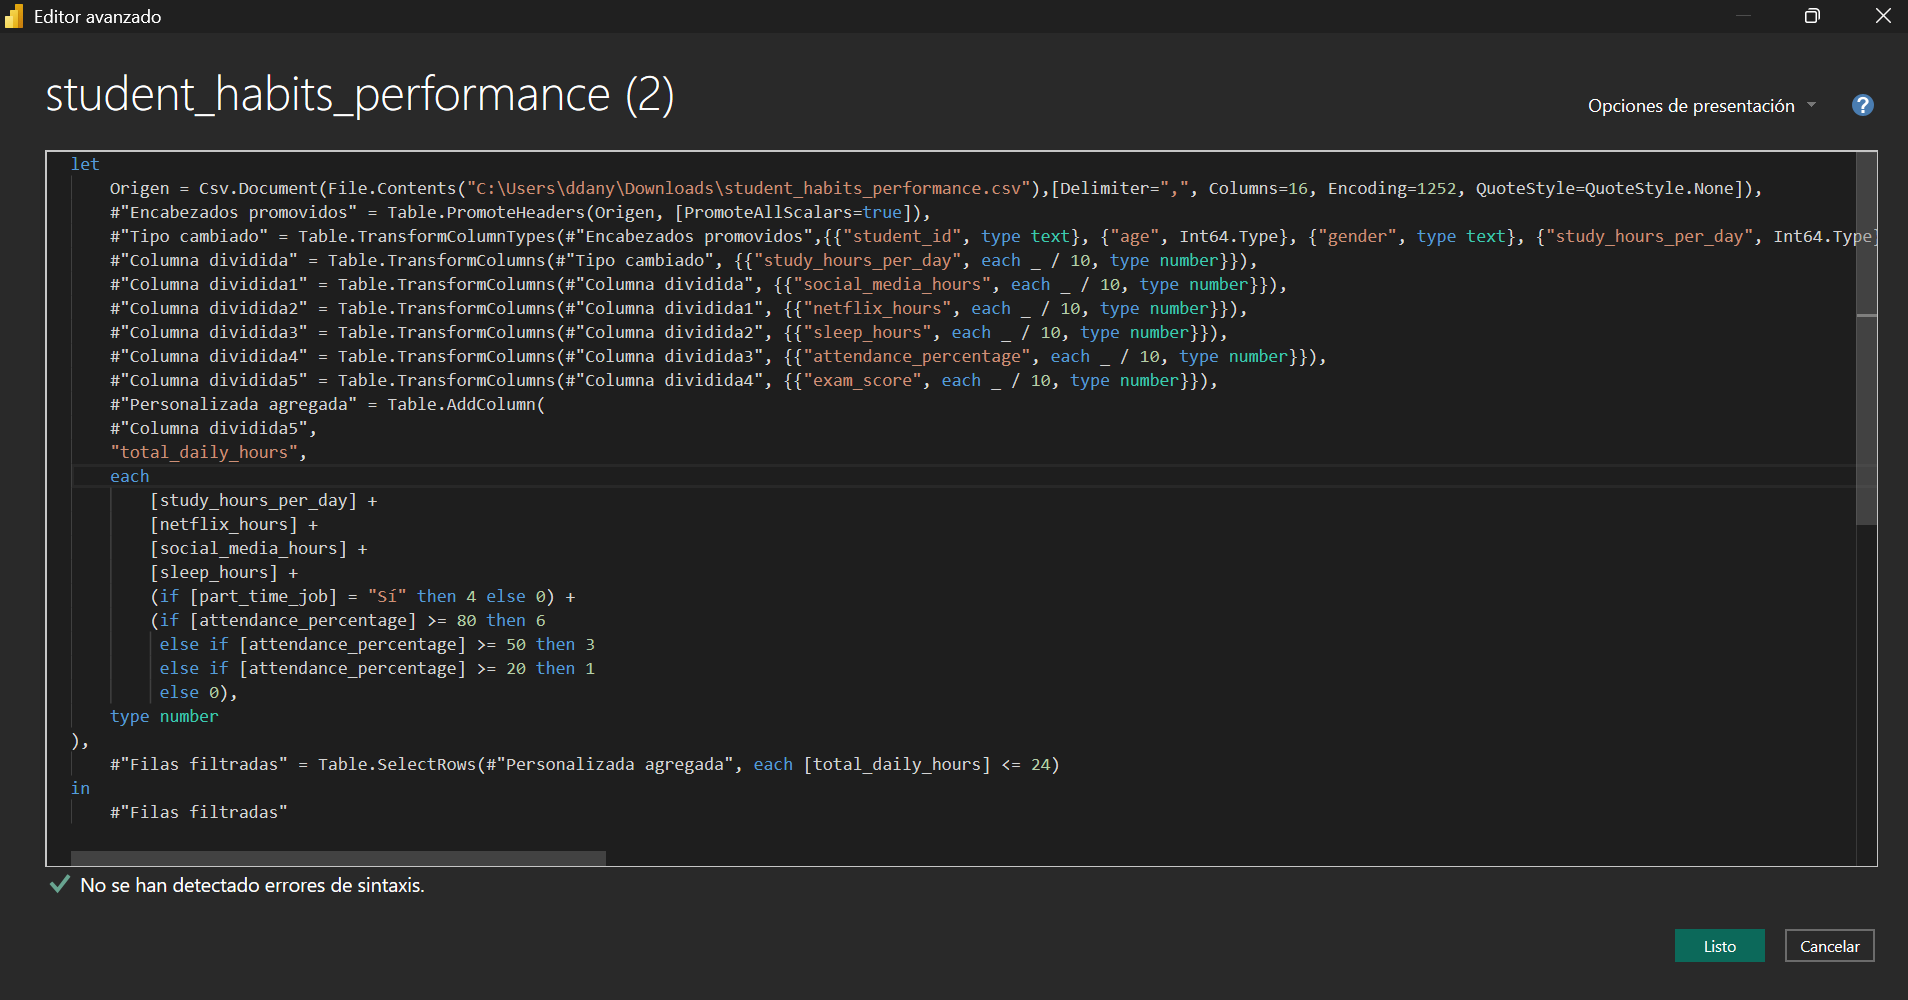
\includegraphics[width=0.9\textwidth]{imagenes/total_daily_hours.png}
    \caption{Transformación de datos en Power BI para el cálculo de \texttt{total\_daily\_hours}.}
\end{figure}



%------------------------------------------------
% PASO 10: ESTABLECER LAS REGLAS DE LOS CÁLCULOS DE LOS DATOS
%------------------------------------------------
\section{Paso 10: Reglas de Cálculo, Métricas y Campos Calculados}

Para obtener insights significativos a partir del dataset de hábitos estudiantiles, se han definido diversas métricas clave (KPIs) y campos calculados, cuya finalidad es transformar variables simples en indicadores compuestos que aporten mayor valor informativo y permitan establecer correlaciones más claras con el rendimiento académico.

A continuación se detallan las reglas de cálculo, transformaciones aplicadas y justificación de cada métrica.

\subsection{Índice de Dedicación Académica (IDA)}

\textbf{Definición:} Representa el compromiso del estudiante con sus estudios, considerando tanto las horas dedicadas al estudio como su nivel de asistencia a clases.

\textbf{Fórmula:}
\(IDA = (Horas De Estudio * 0.6) + (Porcentaje De Asistencia * 0.4)\)

\textbf{Rango:} 0 a 100

\textbf{Tipo de métrica:} Compuesta, cuantitativa continua

\textbf{Justificación:} Combina dos variables directamente relacionadas con el desempeño académico. Se le otorga mayor peso al tiempo de estudio porque implica esfuerzo directo fuera del aula.


\subsection{Índice de Estilo de Vida Saludable (IES)}

\textbf{Definición: }Evalúa el grado de vida saludable del estudiante considerando alimentación, sueño y actividad física.

\textbf{Fórmula:}

\(IES = (Horas De Sueno (estandarizadas) * 0.4) + 
(Frecuencia de Ejercicio (escala 1 a 10) * 0.3) + 
(Calidad de Alimentacion (escala 1 a 10) * 0.3)
\)

\textit{Nota: Las horas de sueño se estandarizan con base en un ideal de 8 horas (valor óptimo). Se asignan pesos según literatura académica sobre salud estudiantil.}

\textbf{Rango:} 0 a 10

\textbf{Tipo de métrica: }Compuesta, cuantitativa continua

\textbf{Justificación: }Estilo de vida saludable ha mostrado fuerte correlación con el rendimiento académico y la salud mental. Este índice permite hacer un seguimiento del bienestar general del estudiante.


\subsection{Índice de Tiempo Recreativo (ITR)}

\textbf{Definición: }Mide la cantidad de tiempo destinado a actividades no académicas ni saludables (tiempo de ocio pasivo).

\textbf{Fórmula:}
\(ITR = Horas en Redes Sociales + Horas de Netflix\)

\textbf{Rango:} 0 a infinito

\textbf{Tipo de métrica:} Cuantitativa continua

\textbf{Justificación:} Altos valores pueden indicar distracción o mal uso del tiempo. Es útil para evaluar el equilibrio vida académica/ocio.



\subsection{Condición de Riesgo Académico (Variable Binaria)}

\textbf{Definición:} Clasifica al estudiante como “en riesgo” si cumple dos o más condiciones de bajo desempeño o estilo de vida negativo.


\textbf{Criterios de riesgo:}
\begin{itemize}
    \item Horas de Estudio menor a 1 hora diaria
    \item Porcentaje de Asistencia menor a 60\%
    \item IES menor a 5
    \item ITR mayor a 6 horas
    \item Puntaje en Examen menor a 50
\end{itemize}

\textbf{Fórmula:}
\(CondicionRiesgo = SI(CondicionesCumplidas >= 2, Sí, No)\)

\textbf{Tipo de métrica:}  Cualitativa nominal

\textbf{Justificación:} Útil para segmentar a los estudiantes y priorizar intervenciones.


\subsection{Ratio de Aprovechamiento del Tiempo (RAT)}

\textbf{Definición:} Proporción del tiempo dedicado a actividades productivas frente al total de horas autorreportadas.

\textbf{Fórmula:}
\(RAT = (Horas de Estudio + Horas de Sueño + Horas de Ejercicio) / (Horas Estudio + Sueño + Redes Sociales + Netflix + Ejercicio)
\)

\textbf{Tipo de métrica:} Cuantitativa continua, ratio

\textbf{Justificación:} Permite evaluar si el estudiante está administrando eficientemente su tiempo.


\subsection{Índice de Apoyo Socioeconómico (IASE)}

\textbf{Definición:} Índice sintético basado en si trabaja, calidad de internet y nivel educativo de los padres.

\textbf{Fórmula:}
\(IASE = (Nivel Educ. Padres * 0.4) + (Calidad Internet * 0.3) - (Trabajo Part-time * 0.3)
\)

\textbf{Trabajo part-time} = 1 si trabaja, 0 si no

\textbf{Nivel educativo y calidad de internet estandarizados} a escala de 1 a 10

\textbf{Tipo de métrica:} Cuantitativa continua

\textbf{Justificación:} Ayuda a medir la influencia del entorno socioeconómico sobre el desempeño.


\subsection{Implementación de Cálculos}
Las métricas serán implementadas mediante:  
\begin{itemize}
    \item Transformación de columnas en Power BI (usando DAX)
    \item Cálculo previo en Python durante el preprocesamiento (para validación)
    \item Visualización en dashboards mediante gráficos comparativos e indicadores de color (rojo-amarillo-verde)
\end{itemize}

\subsection{Ejemplos de Visualización en Power BI}

\begin{itemize}
    \item \textbf{Tarjetas (Cards):} Para IDA, IES, ITR y RAT individuales
    \item \textbf{Segmentación por riesgo académico:} Mediante slicers y filtros para “Sí/No”
    \item \textbf{Gráficos de dispersión:} Comparando IES vs Puntaje en Examen
    \item \textbf{Heatmaps y histogramas:} Para distribución de ITR o IDA en la población
\end{itemize}

\subsection{Consideraciones Éticas y Limitaciones}

\begin{itemize}
    \item Estos cálculos no reemplazan evaluaciones psicológicas ni académicas formales.
    \item Algunos campos calculados usan supuestos de peso relativos (basados en literatura, pero pueden ser ajustables).
    \item El dataset es sintético, por lo tanto, las conclusiones tienen un valor exploratorio.
\end{itemize}


%------------------------------------------------
% PASO 11: IMPLEMENTACIÓN DEL DASHBOARD
%------------------------------------------------
\section{Paso 11: Implementación del Dashboard en Power BI}

\subsection{Diseño del Dashboard}

El diseño general del dashboard está enfocado en explorar factores que influyen en el rendimiento académico, estableciendo correlación entre este último y los hábitos de estudio. Está dividido en una página con secciones que responden a categorías como: género, edad, hábitos, salud, etc., y otra página destinada exclusivamente a la visualización de los KPI, los cuales permiten hacer seguimiento del estado académico de los estudiantes.

\subsection{Elementos Visuales}

\begin{figure}[!ht]
    \centering
    \includegraphics[width=0.8\textwidth]{dashboard1.png}
    \caption{Dashboard exploratorio con segmentación por categorías}
    \label{fig:dashboard1}
\end{figure}

\begin{figure}[!ht]
    \centering
    \includegraphics[width=0.8\textwidth]{dashboard2.png}
    \caption{Identificadores objetivos y cuantificables del rendimiento académico (KPI)}
    \label{fig:dashboard2}
\end{figure}

\textbf El conjunto de gráficos del dashboard permite analizar la influencia de cada variable, como el género, edad, hábitos de estudio, en el rendimiento acádemico. Estos elementos del dashboard proporciona una base que ayudan a identificar patrones que afectan a los estudiantes, detectando áreas de mejora y apoyar toma de decisiones orientadas al éxito académico de los alumnos.

%------------------------------------------------
% PASO 12: CONCLUSIONES Y PROPUESTAS DE MEJORA
%------------------------------------------------
\section{Paso 12: Conclusiones y Propuestas de Mejora}

\subsection{Análisis de los KPI}
[Presentar y analizar los resultados obtenidos para cada KPI]

\subsection{Propuestas de Mejora}
[Establecer propuestas de mejora sobre el proceso intervenido, basadas en los resultados del análisis]

\begin{table}[H]
    \centering
    \begin{tabularx}{\textwidth}{|X|X|X|X|}
        \hline
        \textbf{Propuesta de Mejora} & \textbf{Descripción} & \textbf{Impacto Esperado} & \textbf{Dificultad de Implementación} \\
        \hline
        & & & \\
        \hline
        & & & \\
        \hline
        & & & \\
        \hline
    \end{tabularx}
    \caption{Propuestas de Mejora}
\end{table}

%------------------------------------------------
% CONCLUSIONES GENERALES
%------------------------------------------------
\chapter{Conclusiones Generales}

\section{Resumen del Trabajo Realizado}
[Resumir el trabajo realizado a lo largo del proyecto]

\section{Logros y Resultados Obtenidos}
[Describir los logros y resultados obtenidos con el proyecto]

\section{Dificultades Encontradas}
[Mencionar las dificultades encontradas durante el desarrollo del proyecto y cómo se superaron]

\section{Lecciones Aprendidas}
[Describir las lecciones aprendidas durante el desarrollo del proyecto]

\section{Recomendaciones para Futuros Proyectos}
[Proporcionar recomendaciones para futuros proyectos similares]

%------------------------------------------------
% REFERENCIAS
%------------------------------------------------
\chapter*{Referencias}
\addcontentsline{toc}{chapter}{Referencias}

[Incluir todas las referencias utilizadas en el informe, siguiendo algún estilo bibliográfico estándar como APA o IEEE]

%------------------------------------------------
% ANEXOS
%------------------------------------------------
\chapter*{Anexos}
\addcontentsline{toc}{chapter}{Anexos}

[Incluir cualquier material adicional relevante para el informe, como código, datos adicionales, gráficos complementarios, etc.]

\end{document}